\documentclass[12pt]{article}
\usepackage[utf8]{inputenc}
\usepackage{graphicx}
\graphicspath{{img/}}
\usepackage{multicol}
\usepackage{hyperref}
\usepackage[export]{adjustbox}
\usepackage{subfig}
\usepackage{imakeidx}
\makeindex[columns=1, intoc]

\title{Getting Started with GitHub on Windows 10 Using Git Bash}
\author{Andy Malinsky}
\date{14 February 2019}

\begin{document}
\maketitle
\hfill
\begin{multicols}{3}[\columnsep=1cm]
    \centering
    
\includegraphics[width=3cm]{GitHub-Mark}
\columnbreak
    \centering
    
\includegraphics[width=3cm]{gwindows_logo}
\columnbreak
    \centering
    
\includegraphics[width=3cm]{Windows-10-Icon}
\end{multicols}
\newpage

\tableofcontents
\newpage

\section{Introduction}
\subsection{What is Git and Why Use It?}
Software development projects, especially in industry, are usually maintained by a team of developers. Therefore, it is crucial that each team member is able to contribute to the source code without experiencing overriding conflicts. This is where Git comes in. \textbf{Git}\index{Git} is a distributed version control system. This means that Git can track the changes made to a code base and maintain a history of previous versions of a project. This allows for a more efficient collaborative experience between developers working on the same project in parallel. Git distributes copies of the code between a local machine and a remote server, from file storage locations known as repositories\index{repository}. Local machines are the individual computers of each developer, while remote servers could include cloud based platforms such as GitHub. Developers make changes to the code on their local machine, and then share it with collaborators by pushing their changes to the remote server.

\subsection{What is GitHub?}
\textbf{GitHub}\index{GitHub} is a cloud-based web platform that optimizes version control and collaboration using Git. It provides a user interface for interacting with Git projects, and acts as a remote server for source code. In addition, many developers use GitHub as a software project portfolio, which they can share with potential employers and collaborators.

\subsection{What is Git Bash?}
Git commands are ultimately executed at the command line, and were originally designed for complementary Unix environments, such as Linux or macOS. Windows has a built-in command prompt, but it is not a Unix terminal environment. Although the default Windows command prompt is capable of running Git commands, the use of common Unix commands are not recognized, such as 'ls' (discussed later). \textbf{Git Bash}\index{Git Bash} addresses this as it provides an emulation of the default Unix shell, a command line user interface, known as Bash. 

\subsection{Requirements}
The purpose of this user manual is to demonstrate the process of using Git Bash and GitHub for an individual user experience. Topics and Git commands pertaining to collaboration between multiple users are not covered. It is assumed that you have Windows 10 installed, and that you are familiar with navigating the Windows File Explorer, launching Desktop applications, and running downloaded files from the Internet. This guide is for Git version 2.20.1 or greater.

\section{Setting up the Environment}
\subsection{Download and Install Git}
In order to run Git commands using Git Bash you need to install Git first.
\begin{enumerate}
  \item Open an Internet browser and navigate to the following link: \\
        \href{https://git-scm.com/downloads}{https://git-scm.com/downloads}
  \item Click on \emph{Windows} to download the latest source release.
  \item Run the downloaded file.
  \item Click \emph{Next} for every default selection.
  \item Click \emph{Install}.
\end{enumerate}

\subsection{Create a GitHub Account}
Now you are ready to create a GitHub account.
\begin{enumerate}
    \item Open an Internet browser and navigate to the following link: \\
        \href{https://github.com/join?source=header-home}{https://github.com/join?source=header-home}
    \item Follow the steps to create your free personal account.
    \item Once you have created an account, sign in to GitHub.
\end{enumerate}

\subsection{Configure Your Git Identity\index{Git Identity}}
Now that you have Git installed and a GitHub account created, the next step is to set your username and email address for Git. Note, you must press Enter to run each command in the terminal. You may refer to the Figure captions before typing a command.
\begin{enumerate}
    \item Launch Git Bash from the Windows Start menu.
    \item Type in the following command to set your username:
    \begin{figure}[h!]
        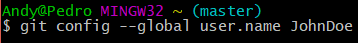
\includegraphics[height=1cm, center]{Git-Config-Name}
        \caption{The value after \emph{user.name} should match your GitHub username.}
    \end{figure}
    \item Type in the following command to set your email:
    \begin{figure}[h!]
        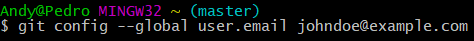
\includegraphics[height=1cm, center]{Git-Config-Email}
        \caption{The value after \emph{user.email} should match the email associated with your GitHub account.}
    \end{figure}
\end{enumerate}

\section{Starting a GitHub Project}
\subsection{Create a New Repository}
Once you are logged in to GitHub you should be able to click the \emph{Start a project} button.
\begin{figure}[h!]
  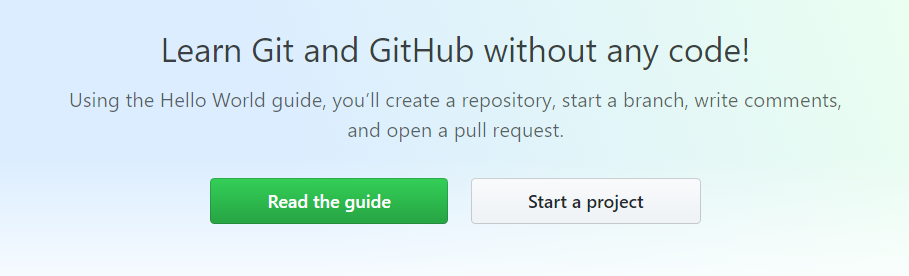
\includegraphics[width=10cm, center]{GitHub-Start-Project}
  \caption{GitHub welcome screen. Find \emph{Start a project} button.}
\end{figure} \\
Next, you will be able to create a new repository. You can always add or edit a Description later. Make sure to check the box to \emph{Initialize this repository with a README} to simplify the process. A README\index{README} file is simply a form of documentation markup that provides information about the project. Once you have filled out the fields click \emph{Create repository}.
\begin{figure}[h!]
  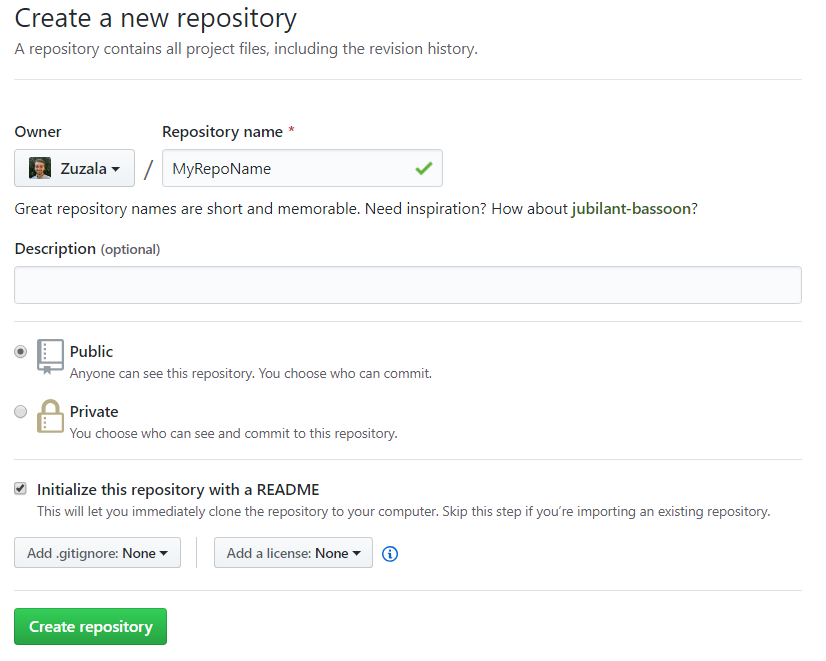
\includegraphics[width=8.5cm, center]{GitHub-Create-Repo}
  \caption{Create a new repository form. First time users may need to verify their email address.}
\end{figure}

\subsection{Clone Your Repository}
Now that you have created a remote location for your repository, you want to have a copy of it on your local machine to make edits on.
    \begin{enumerate}
        \item Using File Explorer, create a new folder where you will keep your GitHub projects.
        \item Next, you want to launch Git Bash and set the current working directory to your GitHub project folder. Here are two ways to do this:
    \end{enumerate}
    \subsubsection{Navigating the Command Line}
    In Git Bash, you want to use the \textbf{cd}\index{\textbf{cd}} command to change directories. If you created your GitHub folder in Documents, the command would be the following:
    \begin{figure}[h!]
        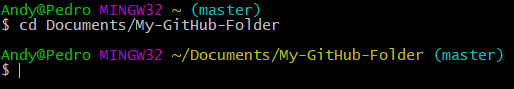
\includegraphics[width=10cm, center]{Bash-cdCommand}
        \caption{Notice the current directory changed.}
    \end{figure}
    \par\bigskip 
    \noindent
    To navigate up, or back, one directory use the \textbf{cd ..} command. Keep this window open as you continue.
    
    \subsubsection{Launch Git Bash from Current Directory Shortcut}
    Another way of changing the working directory is through File Explorer. Open your desired location, right-click, and select \emph{Git Bash Here}.
    \begin{figure}[h!]
        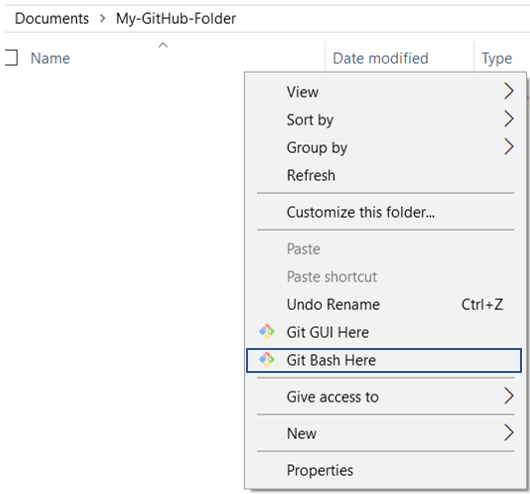
\includegraphics[width=5cm, center]{Bash-Here-Shortcut}
        \caption{This will launch Git Bash with the current directory set to this folder path.}
    \end{figure} \\
    Once you have Git Bash set to your GitHub folder, the next step is to clone your remote repository. 
    \begin{enumerate}
        \item Within your repository on GitHub, click the \emph{Clone or download button}. Then, copy your project's link, as seen in the figure below.
        \newpage
        \begin{figure}[h!]
            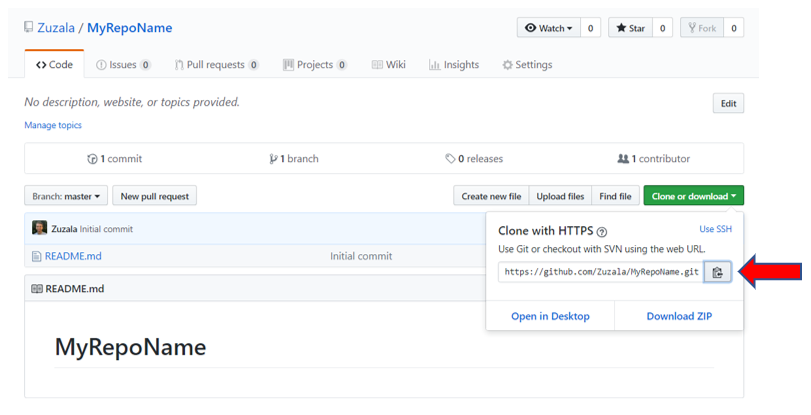
\includegraphics[width=10cm, center]{GitHub-Clone}
            \caption{You can click the clipboard button on the right to copy the link.}
        \end{figure}
        \item In Git Bash, type the following command:
         \begin{figure}[h!]
            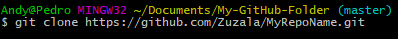
\includegraphics[width=10cm, center]{Git-Clone}
            \caption{You can right-click and select Paste or press Shift+Ins.}
        \end{figure}
        \item Check your folder in File Explorer. \\
        \begin{figure}[h!]
            \centering
            \subfloat{{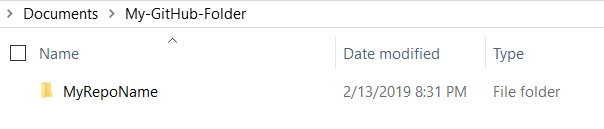
\includegraphics[width=10cm]{File-Explorer-Clone-Folder} }}
            \qquad
            \subfloat{{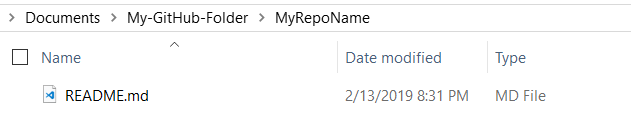
\includegraphics[width=10cm]{File-Explorer-Local-Repo} }}
            \caption{You will now find a local copy of the repository in your folder.}
        \end{figure}
    \end{enumerate}
Now you want to set the current working directory to the cloned folder either by using the \textbf{cd} command in Git Bash or by using the right-click shortcut.
\newpage
\subsection{Tracking and Uploading Changes}
Now you are free to make any changes to your project from your local repository. GitHub supports a wide range of file types, so you can add or create different types of files and folders. The final part of this manual will demonstrate how to upload changes from your local machine to your remote GitHub repository. The three main steps in this process that will be covered are the Add, Commit, and Push commands. 
\begin{enumerate}
    \item You can start by creating a new file in your cloned folder. You may use the following figure as an example of creating a simple text file.
    \begin{figure}[h!]
        \centering
        \subfloat[Right-click and select \newline Text Document.]{{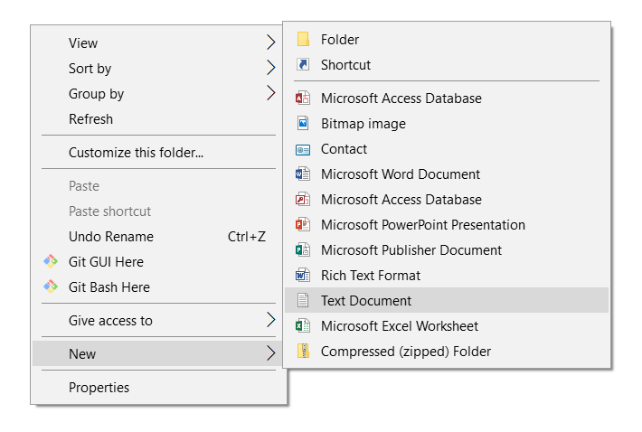
\includegraphics[width=6cm]{Text-File-Shortcut} }}
        \qquad
        \subfloat[Now you should have at least two files in your folder.]{{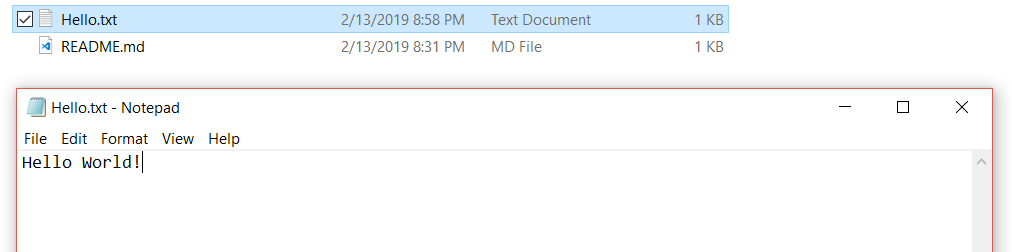
\includegraphics[width=6cm]{File-Explorer-Test-File} }}
        \caption{In the background, Git is tracking your changes.}
    \end{figure}
    \item You can check what files are present in your folder by typing \textbf{ls}\index{\textbf{ls}} in Git Bash.
        \begin{figure}[h!]
            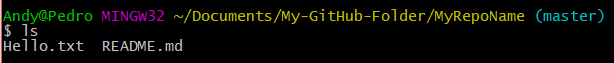
\includegraphics[width=12cm, center]{Git-ls}
            \caption{You will notice all files in the current folder are listed.}
        \end{figure}
    \newpage
    \item You can also check what files were tracked by Git by typing the command \textbf{git status}\index{\textbf{git status}}.
        \begin{figure}[h!]
            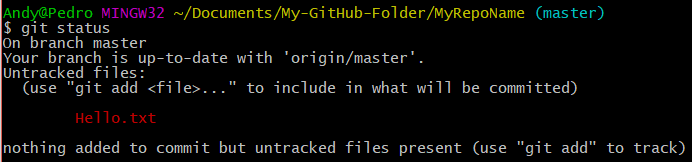
\includegraphics[width=12cm, center]{Git-status}
            \caption{You will notice all edited files are listed in red. This is because they are currently ``untracked''.}
        \end{figure}
    \item \textbf{Add:}\index{\textbf{git add}} Git uses a concept of a staging environment to prepare tracked files to be uploaded. To add files to the staging environment type the following command:
    \begin{center}
       \textbf{git add .} 
    \end{center}
    To track an individual file, for example, you can type \textbf{git add Hello.txt}. You may run \textbf{git status} again and notice newly tracked files listed in green.
    \item \textbf{Commit:}\index{\textbf{git commit}} The next step is to ``commit'' your changes. Git adds the staged files to a commit, a record of changes that is placed among other previous commits, adhering to a version control system. To create a commit type the following command:
    \begin{center}
       \textbf{git commit -m ``Your message about the commit''}
    \end{center}
    You should add a short but meaningful message that describes the changes you made. One example could be ``Added text file''.
    \item \textbf{Push:}\index{\textbf{git push}} The last step is to push your commit by simply typing the following command:
    \begin{center}
       \textbf{git push}
    \end{center}
    \newpage
    \begin{figure}[h!]
        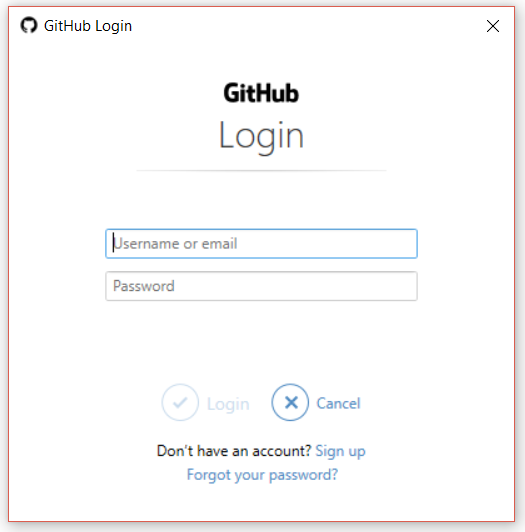
\includegraphics[width=7cm, center]{Git-push}
        \caption{You may be asked to enter your GitHub login credentials for security reasons.}
    \end{figure}
    \item Once you have pushed, refresh your browser to view your changes on GitHub. 
\end{enumerate}

\printindex
\end{document}